\chapter{NOGWs excited by tropopause depressions in 3D}
\label{sec:results3D}
In reality, the PNJ is often observed south of the stormtrack and corresponding tropopause folds during austral winter. The analysis in the next chapter deals with this situation and investigates the impact of meridional aspects on the GW activity in the upper stratosphere.  

Eventually eight full 3D simulations were conducted to investigate the effect of a tilted TD and horizontal wind shear on the meridional propagation of GWs.
Three simulations without horizontal shear an

two effects... meridional shear and tilt of tropopause depression with respect to zonal flow.

\begin{tcolorbox}[]
    (R1) Can the proposed excitation mechanism for NOGWs above tropopause depressions explain the observed GW pattern in ERA5?
    % long vertical wave lengths in vertical cross section and elongated phase line in horizontal
\end{tcolorbox}

\begin{tcolorbox}[]
    (R3) How sensitive are NOGWs from propagating tropopause depressions to the depression's 3D shape and 3D properties of the stratospheric environment?
\end{tcolorbox}

Add another simulation with a stronger PNJ and stronger horizontal shear to observe 

%%% No meridional shear %%%%
\section{Rotating the major axis of the tropopause depression}
\begin{figure*}[tbp]
    \centering
    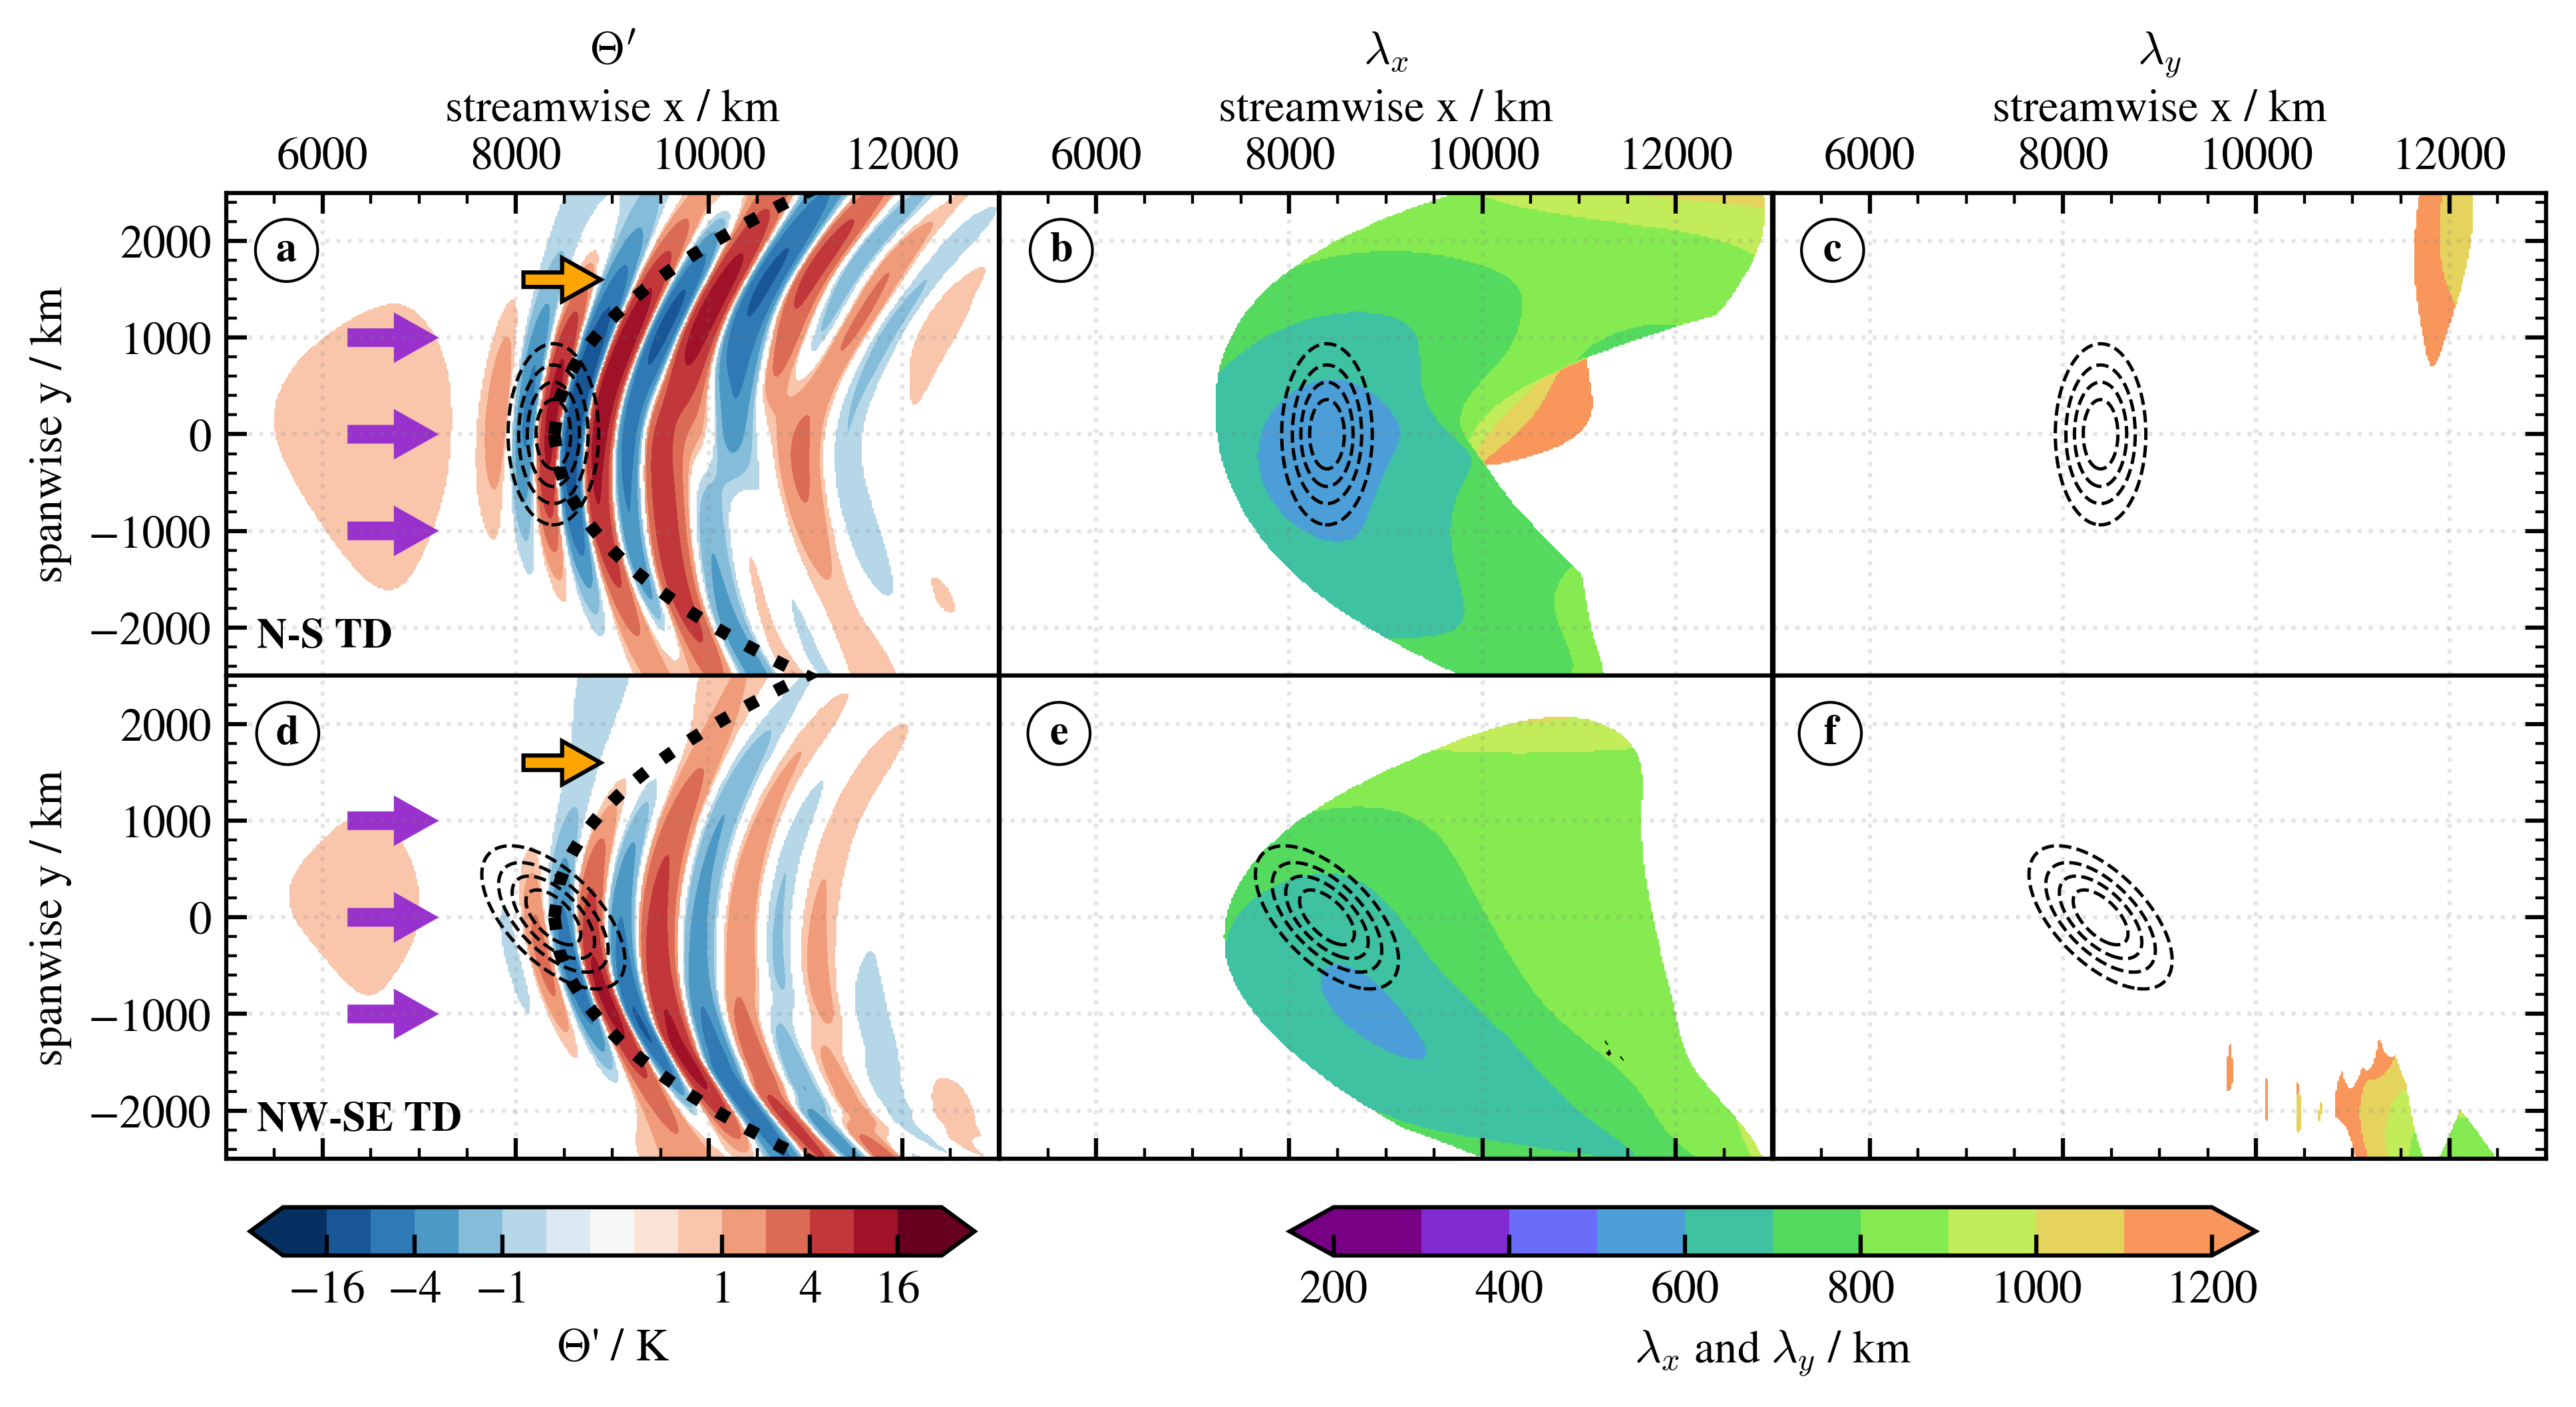
\includegraphics[width=0.99\textwidth]{figures_3D/waveletAna_overview_noShear.png}
    \caption{Horizontal cross sections at 40km above the tropopause for two simulations with no meridional shear as indicated by the purple arrows. Shown are $\theta$', $\lambda_x$ and $\lambda_y$ after 72h. Dominant wavelengths at each grid point are based on a 1-D wavelet analysis in all three dimensions. The first row shows a simulation with a tropopause depression oriented nourth-south, the second row shows a simulation with a tilted depression.}
    \label{fig:waveletAna_noShear}
    % in a barotropic environment
\end{figure*}



%%% PNJ with meridional shear %%%
\section{The influence of meridional shear}
\begin{figure*}[tbp]
    \centering
    \includegraphics[width=0.99\textwidth]{figures_3D/3D-th-referenceSim.png}
    \caption{The "reference" simulation of the entirely 3D simulations with meridional shear. (a),(c) and (e) show horizontal cross sections of $\Theta'$ at z=\SI{40}{\kilo\meter} for three timestamps. (b),(d) and (f) show corresponding meridional cross sections \SI{900}{\kilo\meter} in the lee of the propagating tropopause fold indicated by the dashed black lines in the left figures, too. The purple line in the same figures refers to the location of the PNJ. Meridional cross sections also show zonal wind $u$ and isentropes.}
    \label{fig:3D-reference}
\end{figure*}


\begin{figure*}[tbp]
    \centering
    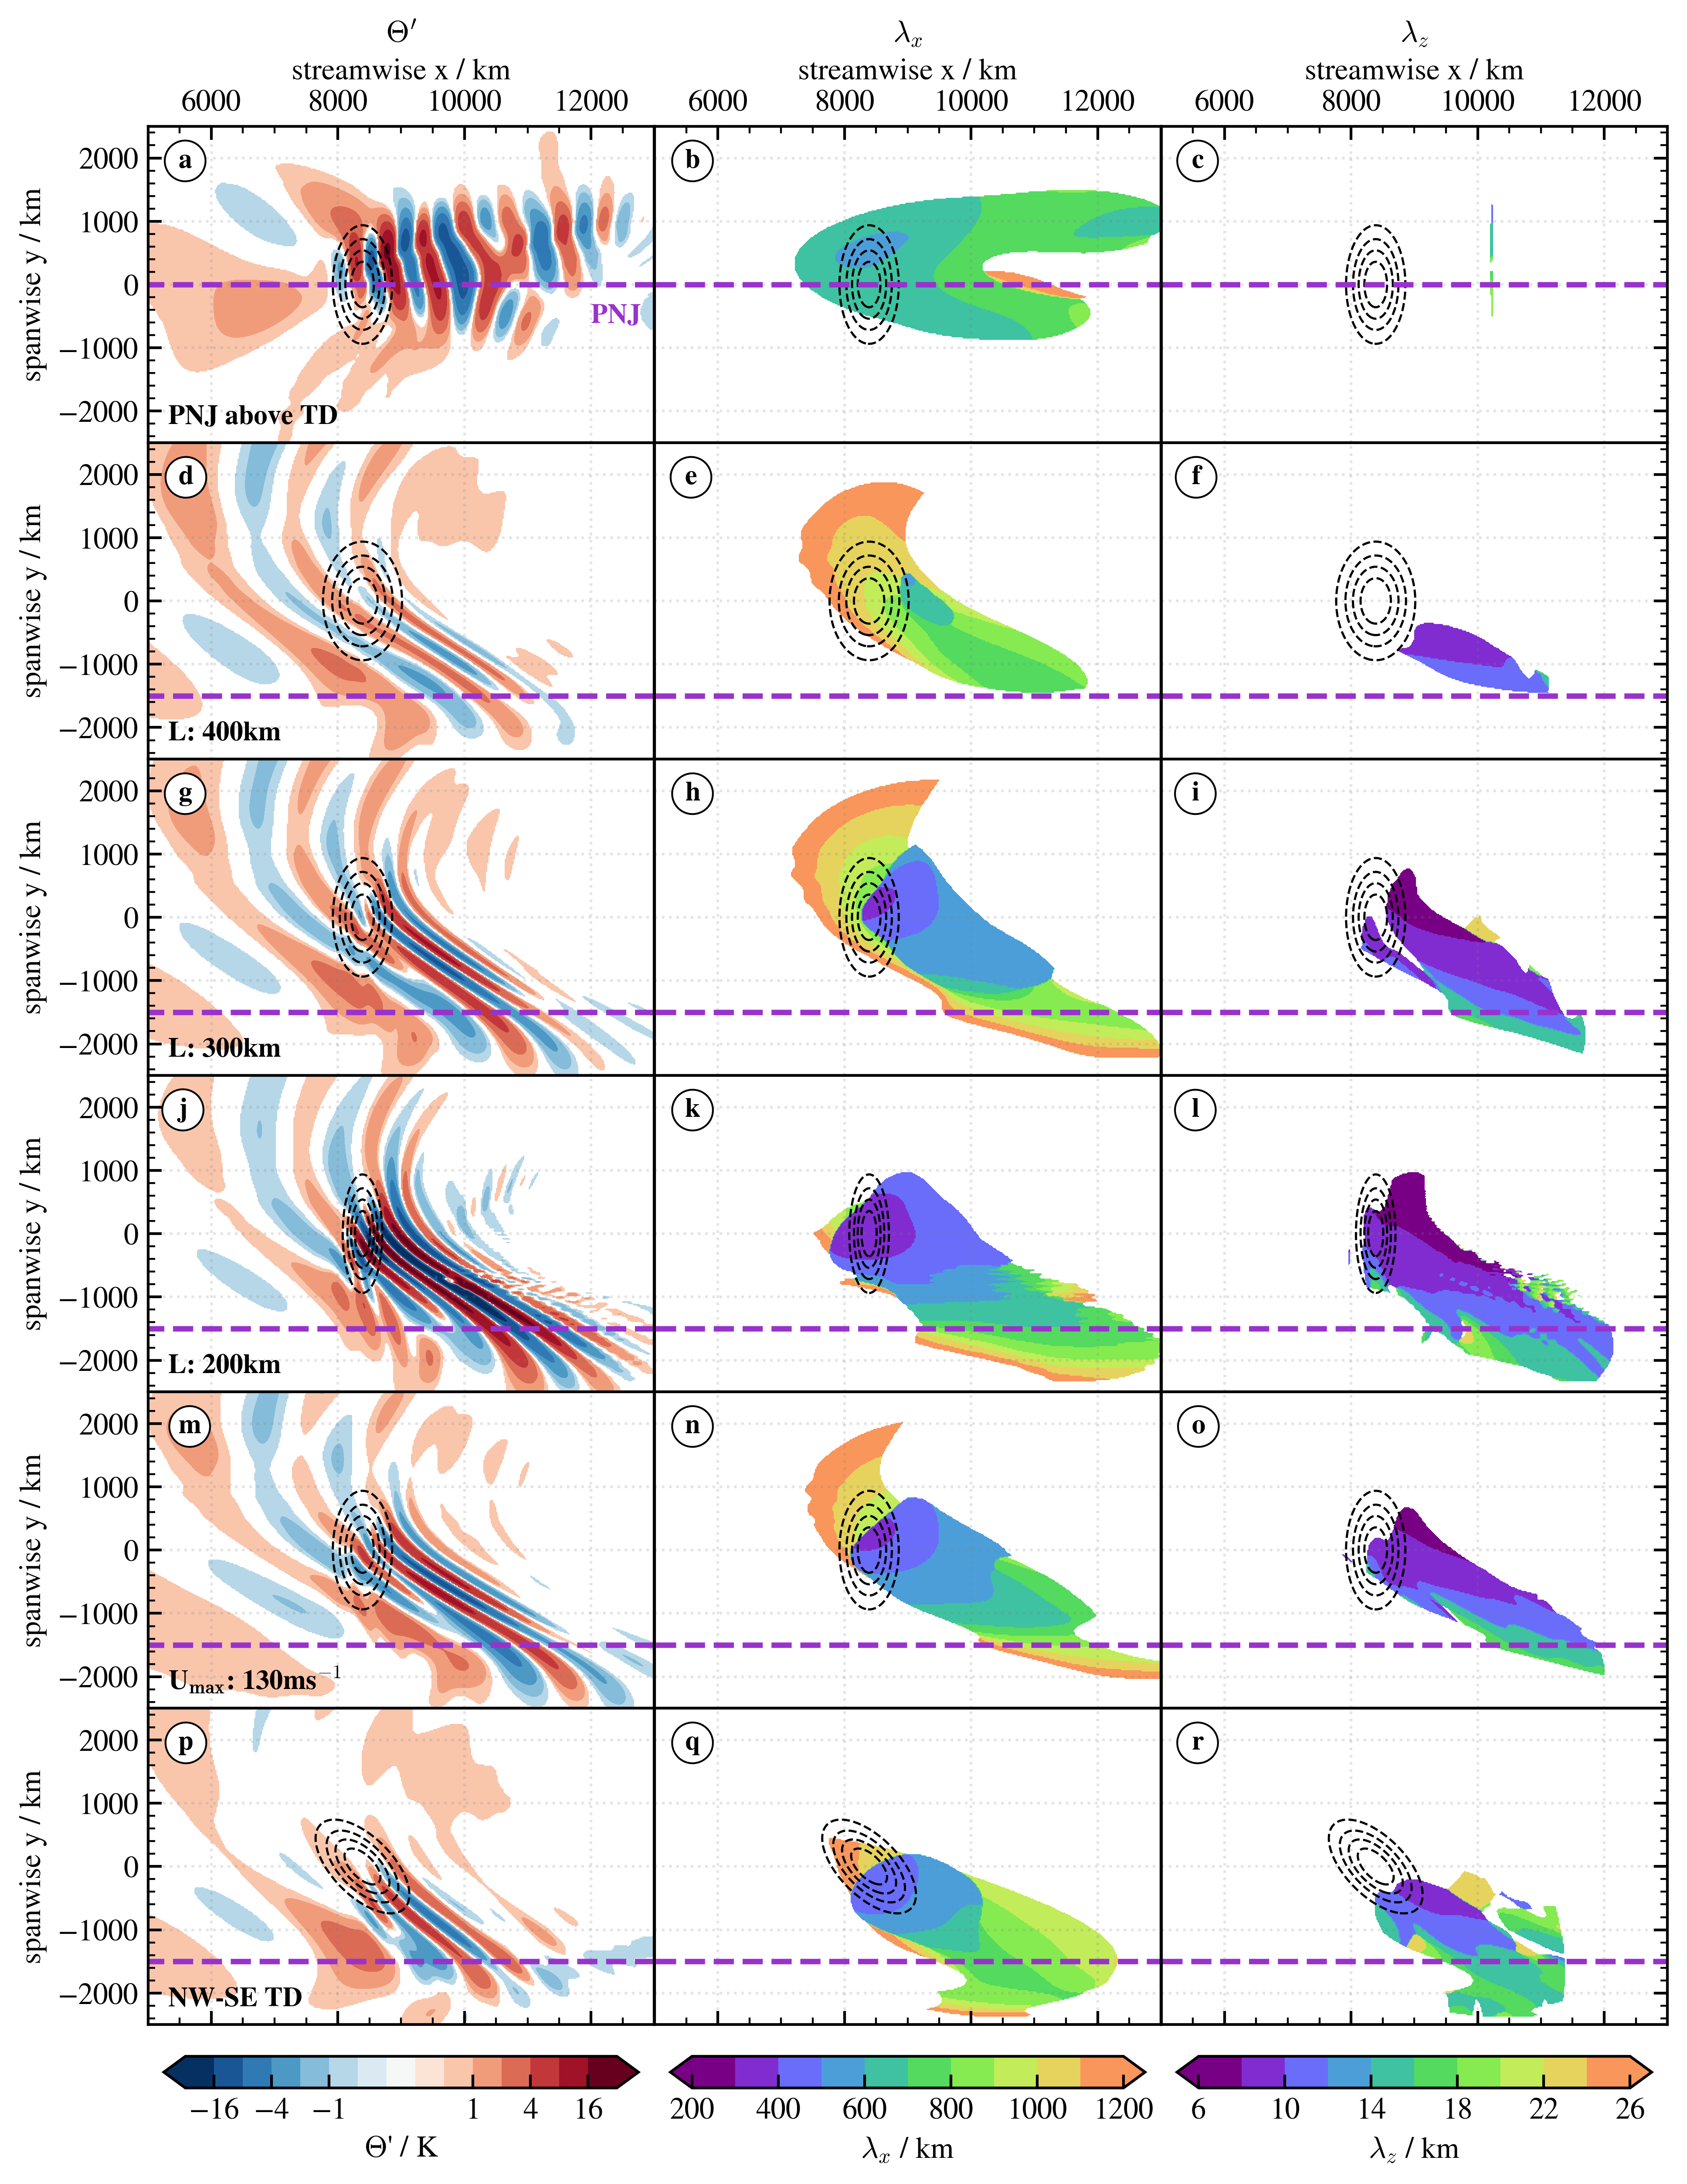
\includegraphics[width=0.99\textwidth]{figures_3D/waveletAna_overview.png}
    \caption{Similiar to Figure \ref{fig:waveletAna_noShear}, but showing simulations with meridional shear as visualized in Figure \ref{fig:wind_profs}b. The horizontal purple line indicates the center of the PNJ. Again, each row refers to a different simulation. Vertical wavelengths from the wavelet analysis at z=\SI{40}{\kilo\meter} are between 6 and \SI{20}{\kilo\meter} for areas without hash pattern in the second and third column.}
    \label{fig:waveletAna}
\end{figure*}
% its effect on the meridional propagation of GWs

Let us recall the equation for the time-dependent meridional wavenumber in a linear framework. The approximation on the right hand side shows two terms that are relevant for the generation of a meridional wave component. The meridional shear $\frac{\partial U}{\partial y}$ and the horizontal wavenumber $k$.


\begin{equation}
    \frac{dl}{dt} = -(k \frac{\partial U}{\partial y} + l \frac{\partial V}{\partial y} + \frac{\beta f}{\hat{\omega}})
    \approx -k \frac{\partial U}{\partial y}.
    \label{equ:meridionalRefraction2}
\end{equation}

1. location of PNJ effects the sign of the du/dy -> sim 1 to all other

2. width of tropopause depression effects k

3. strength of PNJ effects du/dy

4. counterintuitiv effect of orientation of TD... though the orientation favors a southward propagation in the no shear environment... a longer wavelength    effect propagation

\begin{figure*}[tbp]
    \centering
    \includegraphics[width=0.99\textwidth]{figures_3D/3D-EF-MF.png}
    \caption{Similar cross sections as Figure \ref{fig:3D-reference} with horizontal cross sections at z=\SI{40}{\kilo\meter} in (a) and (c) and meridional cross sections in (b) and (d) for x=\SI{9400}{\kilo\meter}, but showing meridional momentum flux MF$_y$ instead of $\Theta'$. The first row is again the 3D "reference" simulation at 72h, the second row is a simulation with similar settings, but here the tropopause depression is tilted by 45°.}
    \label{fig:3D-MFy}
\end{figure*}


% TD's zonal width variation

%% thermal wind balance not fullfilled

extrinsic frequency is conserved along the ray. Is 0 for stationary mountain waves.

intrinsic frequency = 

- Wavelet analysis described earlier

- \cite[]{}




start with linear solution for meridional propagation together with shear...




\section{Momentum flux calculation from an observational perspective}
\label{sec:res3D-sim-vs-obs}
In numerical simulations the vertical flux of horizontal momentum (MF) can be calculated directly from available wind perturbations ($u'$,$v'$ and $w'$) by utilizing equation \ref{equ:mf}. It was used in the preceding sections, too. However, most satellite or ground-based instruments that provide observations of the stratosphere and MLT on a reasonable scale to study GWs are only capable of measuring temperature (e.g. \cite{wu_satellite_1996}, \cite[]{ern_absolute_2004}, \cite{hindley_gravity_2019}, \cite{kaifler_compact_2021}). Temperature perturbations alone allow the calculation of potential energy distributions, but usually momentum flux is the variable of interest to investigate wave-mean flow interactions in the middle atmosphere and constrain GW parameterizations in climate simulations (\cite[]{geller_comparison_2013} or \cite[]{kim_overview_2003}). \\
In this context, \textcite[]{ern_absolute_2004} derived a formulation of MF that depends on the temperature amplitude $\hat{T}$ and the wave's horizontal and vertical wavelength instead of $\overbar{u'w'}$. They start with the expression of the vertical flux of horizontal pseudomomentum valid for conservative wave propagation
\begin{equation}
    (\mathrm{MF}_x, \mathrm{MF}_y) = \bar{\rho} (1-\frac{f^2}{\hat{w}^2}) \Bigl(\overbar{u'w'},\overbar{v'w'}\Bigr) 
    % \approx \bar{\rho}  (\overbar{u'w'},\overbar{v'w'})
    \label{equ:ps-mf}
\end{equation}
(\cite[]{fritts_gravity_2003}). We follow their convention and refer to it as momentum flux MF with MF$_x$ and MF$_y$ being the zonal and meridional MF respectively. They utilize the generally valid linear polarization relations (Equation (14) in \textcite[]{fritts_gravity_2003}) and the dispersion relation
\begin{equation}
    \hat{w}^2 = \frac{N^2 \Bigl(k^2+l^2\Bigr) + f^2 \Bigl(m^2 + \frac{1}{4H^2}\Bigr)}{k^2+l^2+m^2+\frac{1}{4H^2}}
    \label{equ_lid:dispersion_noAss}
\end{equation}
from \textcite[]{fritts_gravity_2003} to end up with
\begin{equation}
    (\mathrm{MF}_x, \mathrm{MF}_y) = A \cdot B \frac{\bar{\rho}}{2} \Bigl(\frac{g}{N}\Bigr)^2 {\Bigl(\frac{\hat{T}}{\bar{T}}\Bigr)^2} \Bigl(\frac{k}{m},\frac{l}{m}\Bigr).
    \label{equ:mf-tp}
\end{equation}
The only assumptions that accompany equation \ref{equ:mf-tp} are a monochromatic wave perturbation and hydrostatic equilibrium. In \textcite[]{ern_absolute_2004} and many follow-up publications (e.g. \cite[]{preusse_characteristics_2014}, \cite[]{ern_gracile_2018}, \cite[]{hindley_gravity_2019}) the factors $A$ and $B$ are neglected by refererring to the midfrequency approximation. NOGWs above tropopause depression can be considered low frequency waves with large horizontal wavelengths. It needs to be checked if $A$ and $B$ are still neglible in this spectral range. While the factor
\begin{equation}
    \begin{split}
        A = &\biggl(1-\frac{\hat{\omega}^2}{N^2}\biggr) \biggl(1 + \frac{1}{m^2} \Bigl(\frac{1}{2H}-\frac{g}{c_s^2}\Bigr)^2\biggr)^{-1} \\
            &\biggl(1+\Bigl(\frac{f}{m \hat{\omega}}\Bigr)^2 \Bigl(\frac{1}{2H} - \frac{g}{c_s^2}\Bigr)^2\biggr)^{0.5}
    \end{split}
    \label{equ:A}
\end{equation}
naturally appears following the approach of \textcite[]{ern_absolute_2004}. The factor
\begin{equation}
    B = \left| \frac{\tilde{\Theta}}{\tilde{T}} \right|^2 = \left| 1 + \frac{1}{\beta} \frac{\gamma-1}{c_s^2} \frac{\hat{\omega}}{\frac{N^2}{g}}i\right|^{-2}
    \label{equ:B}
\end{equation}
with
\begin{equation}
    \beta = -\frac{\hat{\omega}}{N^2-\hat{\omega}^2} \biggl(m + \Bigl(\frac{1}{2H}-\frac{g}{c_s^2}\Bigr)i\biggr)
    \label{equ:beta}
\end{equation}
represents the error by assuming equal amplitudes for $\hat{\Theta}$ and $\hat{T}$ considering all motions to be adiabatic (\cite[]{fritts_gravity_2003} and \cite[]{ern_directional_2017}).
\begin{wrapfigure}{r}{7.5cm}
    \includegraphics[width=7.5cm]{figures_3D/waveletAna_mfcorrection_factor.png}
    \caption{The correction factor A$\cdot$B in equation \ref{equ:mf-tp} for a range of vertical and horizontal wavelengths. It is reproduced from \textcite[]{ern_directional_2017} (supporting information) for a larger $f$ and smaller $c_s$. The dashed rectangle contains all combinations of wavelenghts from the wavelet analysis.}
    \label{fig:mf_correction}
\end{wrapfigure}
In their supporting information \textcite[]{ern_directional_2017} visualize $A$ and $B$ for a common range of vertical and horizontal wavelengths and typical stratospheric values of $N=\SI{0.02}{\per\second}$, $H=\SI{7}{\kilo\meter}$ and $T=\SI{250}{K}$ resulting in $c_s = \SI{316}{\meter\per\second}$. Furthermore, $\gamma=0.4$ and $g=\SI{9.81}{\meter\per\second^2}$. The Coriolis parameter $f$ was chosen for a latitude of 30°. All values are representative for the idealized simulations of this work, but $f$ was a factor of 1.64 larger in the simulations and the background temperature of the isothermal atmosphere was $T=\SI{239}{K}$. Therefore, Figure (S1c) of \textcite[]{ern_directional_2017} is reproduced in Figure \ref{fig:mf_correction} for a Coriolis parameter $f=\SI{1.2e-4}{\per\second}$ (latitude of 55°) and $c_s = \SI{310}{\meter\per\second}$ due to $T=\SI{239}{K}$. \\
Adapting the Coriolis parameter had no noticeable effect. Lowering $c_s$ made $A \cdot B$ smaller, so less negligible, but the factor is still greater than $0.95$ for most combinations of wavelengths appearing in the simulations (dashed rectangle). In general, Figure \ref{fig:mf_correction} clarifies that $A \cdot B$ is much more significant for non-hydrostatic or high frequency waves, while GWs with large horizontal scales are less affected and $A \cdot B$ can be neglected for the following comparison.

At this point, it is important to clarify another relation. \textcite[]{ern_absolute_2004} derived an equation for the momentum flux that depends on the wave's temperature amplitude $\hat{T}$. $\hat{T}$ results from the spectral analysis of the 3D temperature measurements just like horizontal and vertical wavelengths and refers to the amplitude of a perfect sine or cosine wave. These spectral analysis methods improved consistently over the past two decades. Examples are the "S3D" method by \textcite[]{lehmann_consistency_2012} or the work of \textcite[]{wright_exploring_2017} who extended the Stockwell transform to 3D and applied it to new satellite measurements with AIRS (see also \cite[]{hindley_gravity_2019} and \cite[]{hindley_18year_2020}). When following these analysis methods it makes sense to use $\hat{T}$ for calculating MF, because maximum amplitudes might be missed by the coarse resolution of the measurements. In contrast, numerical models provide temperature perturbations $T'$ on a regular grid and it is possible to calculate MF directly via the temperature variance $\overbar{T'^2}$. Again, the overbar denotes averaging over one or multiple full wave cycles. Relating $\overbar{T'^2}$ to $\hat{T}^2$ yields
\begin{equation}
    \overbar{T'^2} = \overbar{\hat{T} sin(\phi)^2} = \frac{1}{2}\hat{T}^2,
    \label{equ:tvariance}
\end{equation}
because $\overbar{sin(\phi)^2} = \frac{1}{2}$. Since temperature variance defines the eddy potential energy per unit mass $E_p$ (first row in equation \ref{equ:epot}), we can use equation \ref{equ:tvariance} to rewrite $E_p$ in terms of $\hat{T}$
\begin{equation}
    \begin{split}
        E_p &= \frac{1}{2} \Bigl(\frac{g}{N}\Bigr)^2 \overbar{\Bigl(\frac{T'}{\bar{T}}\Bigr)^2} \\
            &= \frac{1}{4} \Bigl(\frac{g}{N}\Bigr)^2 \Bigl(\frac{\hat{T}}{\bar{T}}\Bigr)^2
    \end{split}
    \label{equ:epot}
\end{equation}
and relate it to the momentum flux
\begin{equation}
    (\mathrm{MF}_x, MF_y) = \bar{\rho} \Bigl(\frac{g}{N}\Bigr)^2 \overbar{\Bigl(\frac{T'}{\bar{T}}\Bigr)^2} \Bigl(\frac{k}{m},\frac{l}{m}\Bigr) = 2 \bar{\rho} E_p \Bigl(\frac{k}{m},\frac{l}{m}\Bigr)
    \label{equ:mf-epot}
\end{equation}
based on equation \ref{equ:mf-tp} and neglecting the factor $A \cdot B$ (\cite[]{ern_gracile_2018}, \cite*[]{ern_intermittency_2022}). From Figure \ref{fig:mf_correction} it is clear that the factor $A \cdot B$ is neglible for the low frequency GWs excited above tropopause folds, so in the following  we will use equation \ref{equ:mf-epot} to calculate the pseudomomentum flux from temperature perturbations. In a similar manner it is possible to show that the factor $\bigl(1-\frac{f^2}{\hat{\omega}^2}\bigr)$ in equation \ref{equ:ps-mf} can be neglected to calculate the pseudomomentum flux from wind perturbations. Again, the factor is greater than 0.95 for most combinations of horizontal and vertical wavelengths that appear in the idealized simulations, so the vertical flux of horizontal pseudomomentum is underestimated by about \SI{5}{\percent} or less when replaced by the conventional momentum flux $\bar{\rho}(\overbar{u'w'},\overbar{v'w'})$ (equation \ref{equ:mf}) under the midfrequency approximation ($N >> \hat{\omega} >> f$). \\
For a broader understanding we can obtain another perspective on this error by introducing the total energy
\begin{equation}
    E_0 = E_k + E_p = \frac{1}{2} \Bigl(\overbar{u'^2} + \overbar{v'^2} + \overbar{w'^2}\Bigr) + \frac{1}{2} \Bigl(\frac{g}{N}\Bigr)^2 \overbar{\Bigl(\frac{T'}{\bar{T}}\Bigr)^2}
    \label{equ:etot}
\end{equation}
with the kinetic energy per unit mass $E_k$ (e.g. \cite[]{gill_atmosphere-ocean_1982} or \cite[]{tsuda_global_2000}). For non-rotating GWs the kinetic and potential energy tend to be the same ($ E_k \approx E_p$). In that case, the wave energy is equipartiioned and from equation \ref{equ:mf-epot} it follows
\begin{equation}
    \mathbf{MF} = 2 \bar{\rho} E_p \frac{\mathbf{K}}{m} = \bar{\rho} E_{0} \frac{\mathbf{K}}{m}
    \label{equ:mf-etot}
\end{equation}
with the horizontal wavenumber vector $\mathbf{K}$ (compare to \cite[]{andrews_wave-action_1978} or \cite[]{fritts_gravity_2003}). The kinetic energy part becomes more and more dominant for low frequency waves (\cite[]{gill_atmosphere-ocean_1982}), so the error of calculating the pseudomomentum flux under the midfrequency approximation (equation \ref{equ:mf} and \ref{equ:mf-epot}) is proportional to $\frac{E_k}{E_p}$.  

After this extensive discussion on relevant approximations and relations, Figure \ref{fig:mf_scatter} finally compares zonal and meridional MF from wind perturbations to MF from temperature perturbations for all 3D simulations in Figure \ref{fig:waveletAna}.
\begin{figure*}[tbp]
    \centering
    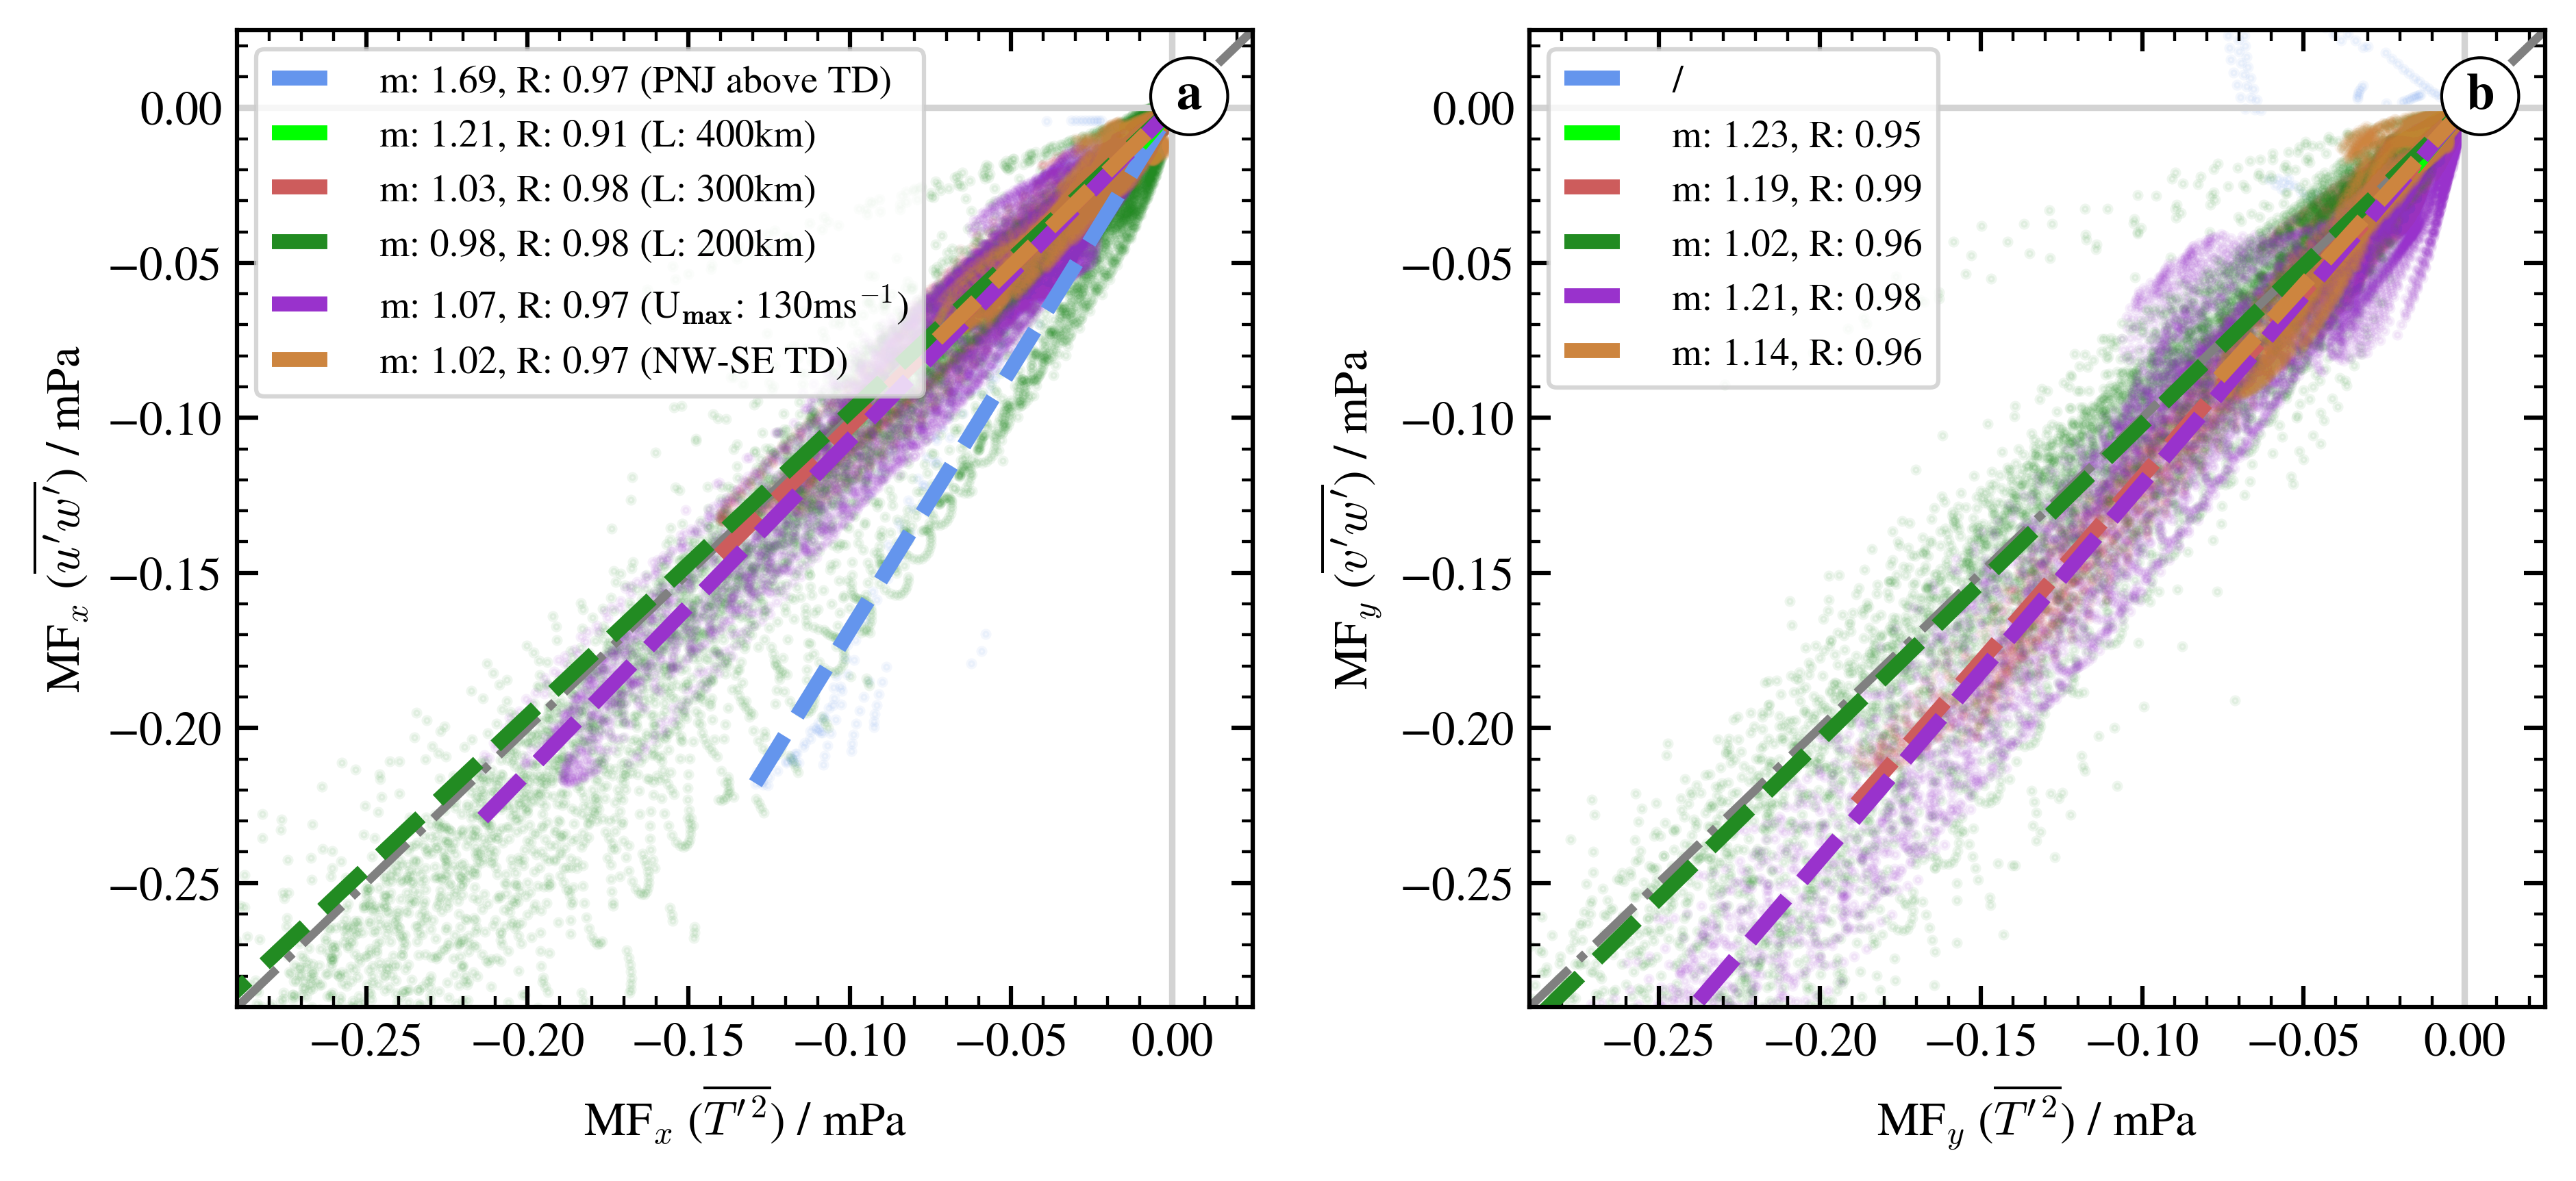
\includegraphics[width=0.99\textwidth]{figures_3D/waveletAna_mf_scatter.png}
    \caption{Scatter plots of the zonal (a) and meridional (b) MF at z=\SI{40}{\kilo\meter} after 72h for all simulations in Figure \ref{fig:waveletAna}. The x-axis refers to the MF calculated from temperature perturbations, the y-axis refers to the MF calculated from wind perturbations. Colored dashed lines are linear fits with slope m and intercept $y_{0}=0$ for each individual simulation.}
    \label{fig:mf_scatter}
\end{figure*}
Overall, momentum fluxes from wind and temperature correlate well. R values are high for all simulations, so linear regressions in Figure \ref{fig:mf_scatter} represent meaningful relations. Especially linear fits of the zonal MF show a good agreement with slope values $m \approx 1$ with one exception. For reasons not fully understood, the slope of the linear regression for the simulation with the PNJ centered above the propagating tropopause depression has a slope of $m \approx 1.7$. In this simulation setup GWs propagate upward into the PNJ without a turning of phase lines resulting in no meridional flux. Nevertheless, we would expect the correlation of the MF$_x$ to be similar to the remaining simulations. \\
MF$_y$ (Figure \ref{fig:mf_scatter}b) also shows good agreement, but a general low bias of temperature-based with respect to wind-based MF can be observed. Only the simulation for the smallest depression width $L=\SI{200}{\kilo\meter}$ has an almost perfect slope while the general picture indicates $15-\SI{25}{\percent}$ higher values for MF$_y$ from winds.\\
MF$_x$ and MF$_y$ suggest a higher correlation for smaller depression widths $L$. Three simulations ($L=400,300,\SI{200}{\kilo\meter}$) are not enough to be conclusive here, but this trend could be related to the effect of rotation that becomes more relevant for wider tropopause folds that result in larger horizontal wavelengths and lower intrinsic frequencies $\hat{\omega}$. As discussed in the beginning of this section, the neglected factor $A \cdot B$ for the MF from $T'$ is not sensitive to large horizontal scales or an increased impact of Coriolis. On the other hand, the factor $\bigl(1-\frac{f^2}{\hat{\omega}^2}\bigr)$ in equation \ref{equ:ps-mf} decreases for smaller $\hat{\omega}$, so MF from wind is overestimated, when this factor is neglected for low frequency waves with $\hat{\omega}$ approaching $f$. Maybe it is this simplification under the midfrequency approximation that becomes less valid and leads to a higher MF from winds for wider tropopause folds.

Despite these uncertainties, we conclude that the calculation of MF from temperature perturbations still leads to meaningful results for the spectrum of GWs excited by propagating tropopause depressions. Considering the uncertainty of real measurements the correspondence between temperature-based and wind-based MF is very good and uncertainties due to the calculation are tolerable. In addition, it shows that the majority of the GWs within the idealized simulations obey the polarization and dispersion relations of GWs and propagate linearly up to an altitude of at least \SI{40}{\kilo\meter}. The analysis of horizontal cross sections at lower levels leads to similar conclusions and is therefore left out.

% zero intercept was used, so larger fluxes might have stronger influence slope value??
% A particularly striking result is a widespread 

% The right part in equation \ref{equ:mf-etot} fits to the work of \textcite[]{andrews_wave-action_1978} or the work of \textcite[]{fritts_spectral_1993} who derived energy spectra in the upper atmosphere from observations. 

% Vertical timeseries of temperature from Lidar observations usually aren't sufficient to derive horizontal momentum fluxes without additional information or assumptions for horizontal wavelengths.
% Gracile paper (Ern 2018) states a factor of Ekin/Epot = 5/3???? should be E0/Epot??
% $f$ is the inertial frequency
% p=5/3 (intrinsic frequency ωˆ spectrum of the GW wave energy density assumed to decrease with ωˆ−5/3)
% The acceleration or deceleration (X, Y ) of the background flow, in the following for simplification called gravity wave drag, is given by the vertical gradient of momentum flux: (X, Y ) = − 1 % ∂ (Fpx, Fpy ) ∂z , (12) with X and Y the drag in the zonal and meridional directions, respectively, and z the vertical coordinate.
 
% F = rho * k/m * Epot,max.
% Es gilt also Etot = Ekin + Epot = Epot,max (in Worten... zum Zeitpunkt, wo die potentielle Energie über die Schwingung maximal wird verschwindet der kinetische Anteil --> Ekin = 0). Wenn wir nun F allein aus den Temperaturvarianzen berechnen wollen nehmen wir an, dass
% Epot {gemittelt über eine Wellenperiode} = Ekin {gemittelt über eine Wellenperiode} (hier kommen dann wohl Annahmen wie linear und non-dissipative mit rein). Daraus folgt dann 
% --> Etot = 2 * Epot {gemittelt über eine Wellenperiode}
% --> F = rho * k/m * 2*Epot {gemittelt über eine Wellenperiode} = rho * k/m *(g/N)^2 * average((T'/T)^2)

\section{Summary and answer to research question (R1) and (R3)}
%\label{sec:res3D-sim-vs-obs}

\begin{tcolorbox}[]
    (R1) Can the proposed excitation mechanism for NOGWs above tropopause depressions explain the observed GW pattern in ERA5?
    % long vertical wave lengths in vertical cross section and elongated phase line in horizontal
\end{tcolorbox}

\begin{tcolorbox}[]
    (R3) How sensitive are NOGWs from propagating tropopause depressions to the depression's 3D shape and 3D properties of the stratospheric environment?
\end{tcolorbox}

Phase lines in vertical cross section triggered the analogy to MWs

It is the southward shift of the PNJ with respect to the propagating tropopause depression that leads to the GW pattern of elongated phase lines observed in the ERA5 data % (Figure \ref{fig:doernbrack_era5_horiz}). 

Same conclusion as many studies that oblique propagation of GW is significant and has to be improved in GCMs. Parameterisations like recent from Eichinger, 

superposition of tilted tropopause fold and meridional shear does not increase MF$_y$, because zonal wavelengths excited by tilted tropopause folds are larger ultimately reducing the meridional flux compared to the same tropopause fold oriented N-S.


%These results provide ad- ditional evidence of a widespread oblique propagation ef- fect, described in an increasing number of studies (Watanabe et al., 2008; Wu and Eckermann, 2008; Preusse et al., 2009; Sato et al., 2009, 2012; Ern et al., 2011; Kalisch et al., 2014; Hindley et al., 2015; Alexander et al., 2016; Ehard et al., 2017). 